\documentclass[11pt]{article}

\usepackage{amsmath, amssymb, fancyhdr, enumitem, mathtools}
\oddsidemargin 0cm \topmargin -2cm \textwidth 16.5cm \textheight 23.5cm \parindent 0pt \parskip 0.5em

% header
\title{Parallel Algorithms for Greedy Graph Coloring}
\date{April 7, 2021}
\author{Sarah Pethani (spethani) and Jeff Tan (jefftan)}

% structure
\newcommand{\question}[3]{\vspace{1em}\qb{Question #1:} #2\vspace{0.5em}\hrule\vspace{0.75em}#3\clearpage\break}
\newcommand{\qop}[2] {\newcommand{#1}{\operatorname{#2}}}
\newcommand{\qdef}[2] {\newcommand{#1}{\qtm{#2}}}


% shortcuts
\newcommand{\qC}{\mathbb{C}}
\newcommand{\qN}{\mathbb{N}}
\newcommand{\qQ}{\mathbb{Q}}
\newcommand{\qR}{\mathbb{R}}
\newcommand{\qZ}{\mathbb{Z}}
\newcommand{\qP}{\mathbb{P}}
\newcommand{\qE}{\mathbf{E}}
\newcommand{\qpow}{\mathcal{P}}
\newcommand{\qbi}{\Leftrightarrow}
\newcommand{\qimp}{\Rightarrow}
\newcommand{\qand}{\wedge}
\newcommand{\qor}{\vee}
\newcommand{\qAnd}{\bigwedge}
\newcommand{\qOr}{\bigvee}
\newcommand{\qint}{\cap}
\newcommand{\quni}{\cup}
\newcommand{\qInt}{\bigcap}
\newcommand{\qUni}{\bigcup}
\newcommand{\qemp}{\varnothing}
\newcommand{\qsub}{\subseteq}
\newcommand{\qsups}{\supseteq}
\newcommand{\qsm}{\setminus}
\newcommand{\qtilde}{\sim}
\newcommand{\qt}{\textrm}
\newcommand{\qtm}{\mathrm}
\newcommand{\qb}{\textbf}
\newcommand{\qi}{\textit}
\newcommand{\qbb}{\mathbf}
\newcommand{\qu}{\underline}
\newcommand{\qof}{\circ}
\newcommand{\qrest}{\restriction}
\newcommand{\qblank}{\sqcup}
\newcommand{\qfrom}{\leftarrow}
\newcommand{\qdx}{\frac d{dx}}
\newcommand{\qpar}[2] {\frac{\partial #1}{\partial #2}}
\newcommand{\qov}{\overline}
\newcommand{\qch}[2] {{#1\choose #2}}
\newcommand{\qinv}{\phantom}
\newcommand{\qd}{\displaystyle}
\newcommand{\qdt}{\textstyle}
\newcommand{\qpr}[1] {\qprob\qpc{#1}}
\newcommand{\qexp}[1] {\qE\qpb{#1}}
\newcommand{\qvar}[1] {\qVar\qp{#1}}
\newcommand{\qcov}[1] {\qCov\qp{#1}}
\qop{\qdim}{dim}
\qop{\qspan}{span}
\qop{\qgcd}{gcd}
\qop{\qdet}{det}
\qop{\qsign}{sgn}
\qop{\qproj}{proj}
\qop{\qinf}{inf}
\qop{\qsup}{sup}
\qop{\qmeas}{meas}
\qop{\qVar}{\qbb{Var}}
\qop{\qCov}{\qbb{Cov}}
\qop{\qprob}{\qbb P}
\qop{\qnotice}{notice}
\qop{\qnegl}{negl}
\newcommand{\qfl}[1] {\left\lfloor #1 \right\rfloor}
\newcommand{\qceil}[1] {\left\lceil #1 \right\rceil}
\newcommand{\qlen}[1] {\left\lVert #1 \right\rVert}
\newcommand{\qabs}[1] {\left| #1 \right|}
\newcommand{\qp}[1] {\left( #1 \right)}
\newcommand{\qpb}[1] {\left[ #1 \right]}
\newcommand{\qpc}[1] {\left\{ #1 \right\}}
\newcommand{\qpa}[1] {\left\langle #1 \right\rangle}
\newcommand{\qmatrix}[1] {\qpb{\begin{matrix} #1 \end{matrix}}}
\newcommand{\qlist}[1] {\begin{enumerate} #1 \end{enumerate}}
\newcommand{\qlista}[1] {\begin{enumerate}[label=(\alph*)] #1 \end{enumerate}}
\newcommand{\qlistn}[1] {\begin{enumerate}[label=\arabic*)] #1 \end{enumerate}}
\newcommand{\qlistb}[1] {\begin{itemize}[label=\textbullet~] #1 \end{itemize}}
\newcommand{\qlistr}[1] {\begin{enumerate}[label=(\roman*)] #1 \end{enumerate}}
\newcommand{\qlistA}[1] {\begin{enumerate}[label=\Alph*.] #1 \end{enumerate}}
\newcommand{\qlistR}[1] {\begin{enumerate}[label=\Roman*.] #1 \end{enumerate}}
\newcommand{\qtable}[2] {\begin{displaymath}\begin{array}{#1} #2 \end{array}\end{displaymath}}
\newcommand{\qalign}[1] {\begin{align*} #1 \end{align*}}
\newcommand{\qalignn}[1] {\begin{align}\setcounter{equation}{0} #1 \end{align}}
\newcommand{\qcenter}[1] {\begin{center} #1 \end{center}}
\newcommand{\qquote}[1] {\begin{quote} #1 \end{quote}}
\newcommand{\qcases}[1] {\begin{cases*} #1 \end{cases*}}
\renewcommand{\mod} {\operatorname{mod}}
\renewcommand{\inf} {\infty}
\renewcommand{\hat} {\widehat}
\renewcommand{\tilde} {\widetilde}

\begin{document}                        

\thispagestyle{plain}
\maketitle

\section{Summary}
We are going to implement different parallel algorithms for greedy graph coloring in OpenMP and possibly CUDA. We will analyze/compare their performance, speedup, and solution quality (e.g. does one algorithm use less colors than another).

\section{Background}
Minimal graph coloring is the assignment of colors to the vertices on a graph, such that no two neighboring vertices are assigned the same color. Graph coloring is an NP-hard problem, with applications in job scheduling, register allocation, and many similar problems that are modelable using conflict graphs. For this reason, heuristic algorithms have been developed that make the trade-off between runtime and solution quality. However, many simple greedy approaches to graph coloring are inherently sequential due to dependencies on the colors of existing nodes in the graph.\\

One such algorithm is the sequential greedy algorithm, which iterates through all vertices and assigns to each vertex the smallest available color that is not shared by any neighbors. While this algorithm is easy to implement and has good sequential performance, it does not produce an optimal solution, and is also very difficult to parallelize due to the explicit time dependency between vertex colors.

$$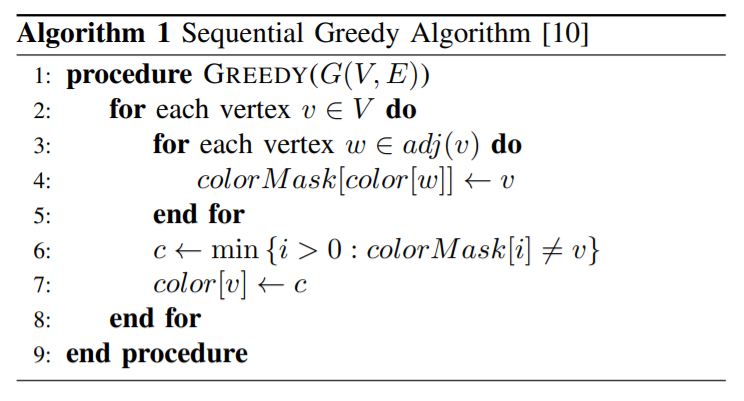
\includegraphics[scale=0.35]{proposal_greedy.png}$$

Two alternative greedy graph coloring algorithms have been proposed to address these issues: the Jones-Plassman (JP) and Gebremedhin-Manne (GM) algorithms.\\

The JP algorithm attempts to parallelize the graph coloring problem by iteratively finding independent sets of uncolored vertices, and coloring these vertices in parallel. At each step, each remaining uncolored vertex is assigned a random number, and all vertices whose numbers are a local maximum are colored the next available color. This process repeats until all vertices are colored. Since the computation at each vertex depends only on its neighbors, vertices can be operated on in parallel as long as there is a mechanism for communication between neighbors.

$$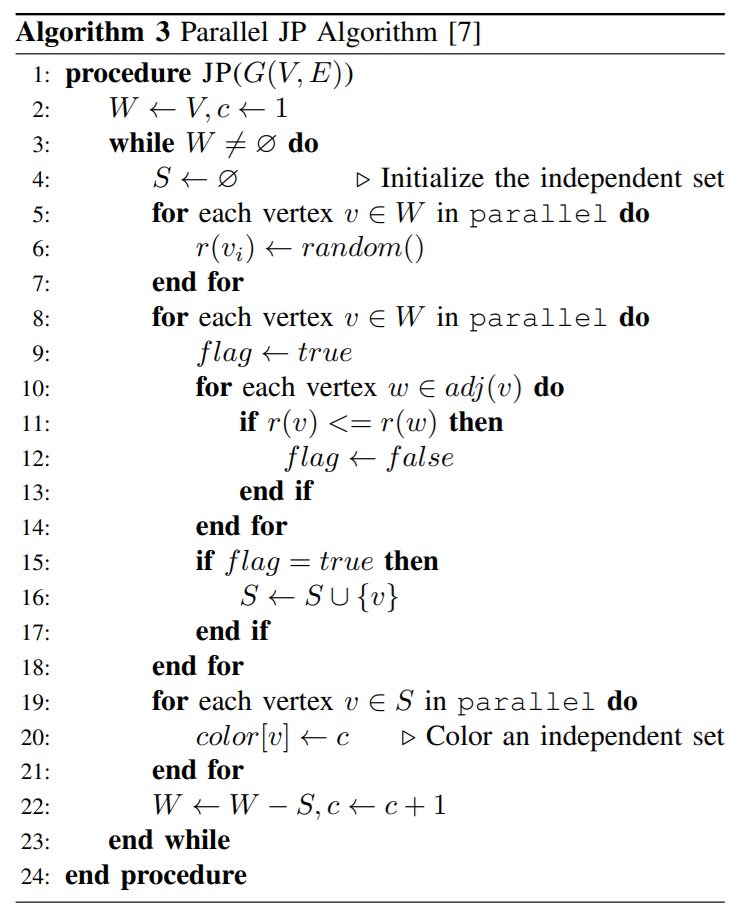
\includegraphics[scale=0.35]{proposal_jp.png}$$

The GM algorithm is a speculative approach that attempts to color as many vertices as possible in parallel, potentially resulting in some conflicts in neighboring vertex colors, which are later resolved.  This algorithm has looser restrictions in terms of deciding when to color in a vertex as compared to the JP algorithm, but as a result, has a backtracking aspect to solve problems caused by the looser restrictions. 

$$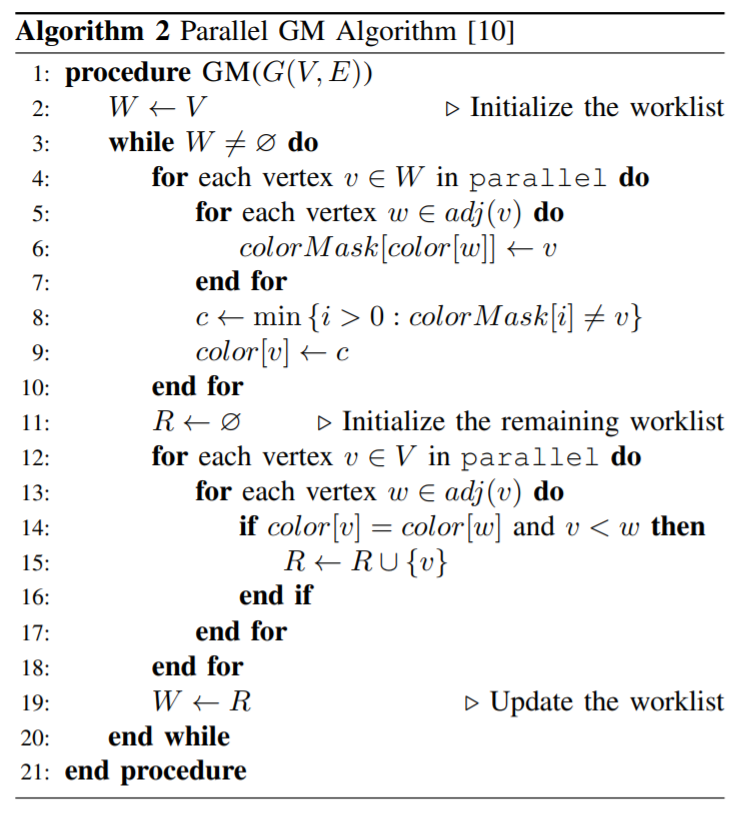
\includegraphics[scale=0.35]{proposal_gm.png}$$

\section{Challenge}
Though the pseudocode for the Jones-Plassman and Gebremedhin-Manne algorithms seem simple at first glance, there is often need for synchronization in terms of creating new sets of vertices that have yet to be colored by the algorithm. In the JP algorithm, we cannot run another iteration of the main outside loop before all of the threads have completed the previous iteration. There is also a need for updating shared memory which needs to be atomic between different threads. For example, each thread must atomically update the graph at the end of each iteration.

Additionally, the pseudocode for these two algorithms assumes the use of sets for representing groups of vertices. We will have to decide if it is better to use built-in C++ sets or if we should have our own implementation which takes into consideration the characteristics of the coloring problem. 

The workload of different threads is not necessarily balanced. In the GM algorithm, if one vertex shares a color with any of its neighbors, we will have to complete additional updates to the vertex set to resolve these conflicts, while other threads will also be contending for access to this vertex set. In addition, since the topology and characteristics of the input graph are unknown, some threads may end up taking much longer than others if we choose a simple static assignment.

\section{Resources}
We will be using the Gates machines and the Lateday clusters to measure performance and speedup. Additionally, we will be referring to https://chenxuhao.github.io/docs/ipdpsw-2016.pdf for the pseudocode of the different greedy coloring algorithms. We will be writing our code from scratch.

\section{Goals and Deliverables}
We plan to achieve implementations of Jones-Plassmann and Gebremedhin-Manne in OpenMP along with analysis of their performance and speedup on both the Gates and Latedays machines. We also plan to implement the sequential greedy algorithm in C++ as a baseline for comparison.

We hope to achieve (as a stre implementations of the two parallel algorithms in CUDA and compare the performance and speedup to the OpenMP implementations. 

From this, we plan to learn if a parallel backtracking algorithm such as GM outperforms a straightforward parallel implementation such as JP. We also hope to learn about any potential tradeoffs in terms of synchronization requirements, communication requirements, ease of work distribution, and solution quality (how minimal is the coloring).  

We plan to report the resulting performance, speedup, and solution differences of both parallel algorithms on varying types of graphs. We will also report any conclusions made about the tradeoffs between the algorithms based on this data.

\section{Platform Choice}
We choose to complete this project using OpenMP (and maybe CUDA) as they provide a more intuitive approach when using shared memory and parallelizing over iterations of a loop. 

\section{Schedule}
\qlistb{
	\item Week 1 (4/14):
	\qlistb{
		\item Implement sequential baseline and begin implementations of Jones-Plassman and Gebremedhin-Manne.
	}
	\item Week 2 (4/21):
	\qlistb{
		\item Finish basic implementations of Jones-Plassman and Gebremedhin-Manne in OpenMP. 
		\item Start writeup for checkpoint.
	}
	\item Week 3 (4/28):
	\qlistb{
		\item Start analyzing performance and speedup of the two algorithms. 
		\item Optimize implementations of Jones-Plassman and Gebremedhin-Manne to have better workload balance, less communication, and less memory contention.
	}
	\item Week 4 (5/5):
	\qlistb{
		\item Generate final data for performance, speedup, and solution quality of the different implementations. 
		\item Create a final poster and report. 
	}
}

\end{document}